\documentclass[cs4size,a4paper]{ctexart}   

\usepackage{cite}
\usepackage{url}
%===数学符号公式===
\usepackage{amsmath}    					% AMS LaTeX宏包
\usepackage[style=1]{mdframed}
\usepackage{amsthm}
\usepackage{amssymb}
\usepackage{bm}                      	% 数学公式中的黑斜体
\usepackage{bbm}
\usepackage{amsfonts}
\usepackage{mathrsfs}                	% 英文花体字 体
\usepackage{bbding,manfnt}    			% 一些图标,如 \dbend
\usepackage{lettrine}                	% 首字下沉,命令\lettrine
\def\attention{\lettrine[lines=2,lraise=0,nindent=0em]{\large\textdbend\hspace{1mm}}{}}
\usepackage{longtable}
\usepackage{enumerate}
\usepackage[toc,page]{appendix}
\usepackage{geometry}         			% 页边距调整
\geometry{top=3.0cm,bottom=2.7cm,left=2.5cm,right=2.5cm}
\usepackage[colorinlistoftodos,prependcaption,textsize=small]{todonotes}
%===公式按章编号===
\numberwithin{equation}{section}
\numberwithin{table}{section}
\numberwithin{figure}{section}
%===基本格式预置===
\usepackage{fancyhdr}
\pagestyle{fancy}
\fancyhf{}  
\fancyhead[C]{\zihao{5}  \kaishu 自动化科学导论课程报告}
\fancyfoot[C]{~\zihao{5} \thepage~}
\renewcommand{\headrulewidth}{0.75pt} 
\CTEXsetup[format={\centering\bfseries\zihao{-2}},name={第, 章}]{section}
\CTEXsetup[nameformat={\bfseries\zihao{3}}]{subsection}
\CTEXsetup[nameformat={\bfseries\zihao{4}}]{subsubsection}
%===图形支持宏包===
\usepackage{graphicx}        			% 嵌入png图像
\usepackage{subfigure}
\usepackage{float}
\graphicspath{{figure/}}
\usepackage{color,xcolor}     			% 支持彩色文本、底色、文本框等
\usepackage[colorlinks,linkcolor=blue,anchorcolor=blue,citecolor=blue]{hyperref}
%\usepackage{caption}
\usepackage[ruled,linesnumbered]{algorithm2e}
%\captionsetup{figurewithin=section}
%===源码和流程图===
\usepackage{listings,fontspec}         	% 粘贴源代码
\newfontfamily\consolas{Consolas}
\definecolor{mygreen}{rgb}{0,0.6,0}
\definecolor{mygray}{rgb}{0.5,0.5,0.5}
\definecolor{mymauve}{rgb}{0.58,0,0.82}
%===颜色===
\usepackage{color,xcolor}
\definecolor{dkgreen}{rgb}{0,0.6,0}
\definecolor{gray}{rgb}{0.5,0.5,0.5}
\definecolor{mauve}{rgb}{0.58,0,0.82}
\usepackage{xcolor}
\lstset{ %
%numberstyle=\tiny\monaco,
%numberstyle=\color[RGB]{0,192,192},
%backgroundcolor=\color{white},   		% choose the background color
backgroundcolor=\color[RGB]{245,245,244},
%backgroundcolor=\color[rgb]{1,1,0.76},
basicstyle=\footnotesize\consolas,       % size of fonts used for the code
identifierstyle=\footnotesize\consolas, 
columns=fullflexible,
breaklines=true,                 		% automatic line breaking only at whitespace
captionpos=b,                    		% sets the caption-position to bottom
tabsize=2,
commentstyle=\color{mygreen}\consolas,   % comment style
%commentstyle=\it\color[RGB]{0,96,96},
escapeinside={\%*}{*)},          		% if you want to add LaTeX within your code
keywordstyle=\color{blue}\consolas,      % keyword style
stringstyle=\color{mymauve}\consolas,    % string literal style
%stringstyle=\rmfamily\slshape\color[RGB]{128,0,0},
frame=single,
rulesepcolor=\color{red!20!green!20!blue!20},
%identifierstyle=\color{red},
language=c++,
framexleftmargin=1.9mm,
xleftmargin=0.4em,
frame=none,
showstringspaces=false,
numbers=none,
}

%--------------------
\hypersetup{hidelinks}
\usepackage{booktabs}  
\usepackage{shorttoc}
\usepackage{tabu,tikz}
\usepackage{float}
\usepackage{multirow}

\tabcolsep=1ex
\tabulinesep=\tabcolsep
\newlength\tikzboxwidth
\newlength\tikzboxheight
\newcommand\tikzbox[1]{%
        \settowidth\tikzboxwidth{#1}%
        \settoheight\tikzboxheight{#1}%
        \begin{tikzpicture}
        \path[use as bounding box]
                (-0.5\tikzboxwidth,-0.5\tikzboxheight)rectangle
                (0.5\tikzboxwidth,0.5\tikzboxheight);
        \node[inner sep=\tabcolsep+0.5\arrayrulewidth,line width=0.5mm,draw=black]
                at(0,0){#1};
        \end{tikzpicture}%
        }
\makeatletter
\def\hlinew#1{%
  \noalign{\ifnum0=`}\fi\hrule \@height #1 \futurelet
   \reserved@a\@xhline}
   
\usepackage{CJK}
\usepackage{ifthen}
\newcommand{\HRule}{\rule{\linewidth}{0.5mm}}
\newcommand{\tabincell}[2]{\begin{tabular}{@{}#1@{}}#2\end{tabular}}%
%===使得公式随章节自动编号===
\makeatletter
\@addtoreset{equation}{section}
\makeatother
\renewcommand{\theequation}{\arabic{section}.\arabic{equation}}
%-------------------------
\usepackage{pythonhighlight}
\usepackage{tikz}                    
\usepackage{tikz-3dplot}
\usetikzlibrary{shapes,arrows,positioning}
%===正文开始===
\begin{document}
%===定理类环境定义===
\newtheorem{example}{例}              	% 整体编号
\newtheorem{algorithem}{算法}	
\newtheorem{theorem}{定理}            	% 按section编号
\newtheorem{definition}{定义}
\newtheorem{axiom}{公理}
\newtheorem{property}{性质}
\newtheorem{proposition}{命题}
\newtheorem{lemma}{引理}
\newtheorem{corollary}{推论}
\newtheorem{remark}{注解}
\newtheorem{condition}{条件}
\newtheorem{conclusion}{结论}
\newtheorem{assumption}{假设}
%===重定义===
\renewcommand{\contentsname}{目录}     
\renewcommand{\abstractname}{摘要} 
\renewcommand{\refname}{参考文献}     
\renewcommand{\indexname}{索引}
\renewcommand{\figurename}{图}
\renewcommand{\tablename}{表}
\renewcommand{\appendixname}{附录}
\renewcommand{\proofname}{证明}
%\renewcommand{\algorithm}{算法} 
\renewcommand\emph[1]{\textcolor{black}{\textbf{#1}}}
%===封皮和前言===
\begin{titlepage}
\begin{center}
% Upper part of the page

\includegraphics[width=0.30\textwidth]{logo}\\[1cm]    
\textsc{\Large Beijing University of Chemical Technology}\\[1.0cm]
\textsc{\Large Computing Methods}\\[0.5cm]
% Title
\HRule \\[0.8cm]
{\huge \bfseries 自动化科学导论课程报告}\\[0.4cm]
\HRule \\[0.7cm]
% Author
\textsc{李昊}
\tableofcontents 
\vfill
% Bottom of the page
{创建日期:2020年3月25日}\\
{更新日期:\today}
\end{center}
\end{titlepage}
\pagestyle{plain}
\pagenumbering{Roman}
\thispagestyle{empty}
%===正文===
\pagestyle{fancy}
\pagenumbering{arabic}



%===第一章===
\section{自动化大类各专业之间的相互关系}
其实吧,说专业差距大,其实也没那么大。举图像识别做例子:大家都做图像识别,可能在研究生阶段区别比较大,但是
对于本科来说差别真的几乎没有。
如果一定要做区分的话
\begin{itemize}
        \item 自动化:偏向系统集成,控制算法,感知算法
        \item 测控:就我们学校,MEMS无疑
        \item 通信:各种雷达信号处理
\end{itemize}

%===第二章===
\section{学习的总结,体会和感受}
\subsection{学习的总结}
自动化学科是一门多学科交叉的高技术学科。研究内容广,几乎无所不包。但是,控制、信息、系统是其核心。自动化学科知识
体系中的核心知识是:控制与智能、对象和建模、系统和工程等三个知识领域,也是自动化学科与其他学科的最重大区别。
\subsection{学习的体会}
选自动化就对了!选自动化就对了!选自动化就对了!千万不要搞过程控制!千万不要搞过程控制!千万不要搞过程控制!
更加坚定了自己选择自动化和进行移动机器人以及机器人感知相关方向研究的意志。
\subsection{学习的感受}
与其说选择专业,我觉得更应该选择研究方向后再决定专业,因为每个专业的研究方向都有很大的重叠部分。

%===第三章===
\section{相关专业方向:同步定位与地图构建(SLAM)}
\subsection{AGV的导航(Navigation)}
导航技术是AGV技术的研究核心,没有导航功能的AGV系统是很难想象的。举个例子,如果AGV系统想要在工厂等工作场所运输货物,
它必须要在不触碰到任何障碍物的情况下运动到不同的地点。
随着信息化技术的提升,CPU算力的提升和传感器的升级,AGV的柔性路径导航吸引了越来越多的研究者进行研究,产业化应用越来越广。
柔性路径导航技术应用较多的是视觉与激光导航、惯性(IMU)导航\cite{5670227}、基于WIFI/UWB等无线信号定位\cite{4380919}的导航技术等。
机器人实现其自主导航的前提是机器人自身位姿的确定,出于对定位精度的要求以及现实环境的复杂化,
目前大多数导航系统都是由上述两种或者多种导航方式的结合组合导航技术\cite{7916260}。

\subsection{SLAM定义}
同步定位与地图构建(SLAM或Simultaneous localization and mapping)是一种概念:希望机器人从未知环境的未知地点出发,在运动过程中通过重复观测到的地图特征(比如,墙角,柱子等)定位自身位置和姿态,再根据自身位置增量式的构建地图,从而达到同时定位和地图构建的目的。

在误差和噪音条件下,定位和地图构建技术上的复杂度不支持两者同时获得连续的解。即时定位与地图构建(SLAM)是这样一个概念:把两方面的进程都捆绑在一个循环之中,以此支持双方在各自进程中都求得连续解;不同进程中相互迭代的反馈对双方的连续解有改进作用。

同步定位与地图构建(SLAM)被定义为以下问题:在建立新地图模型或者改进已知地图的同时,在该地图模型上定位机器人。实际上,这两个核心问题如果分开解决,将毫无意义;必须同时求解。
即通过控制数据$u_{1:t}$和观测数据$z_{1:t}$来求解位姿和地图的联合概率分布
\begin{align}
    p\left(x_{1: t}, m | z_{1: t}, u_{1: t-1}\right)
\end{align}

\subsection{V-SLAM的框架与分类}
视觉SLAM由前端(视觉里程计)、后端(位姿优化)、回环检测、建图4个部分组成。
\begin{itemize}
        \item  视觉里程计 (Visual Odometry):仅有视觉输入的姿态估计\cite{1315094}
        \item 后端优化 (Optimization): 后端接受不同时刻视觉里程计测量的相机位姿,以及闭环检测的信息,对它们进行优化,得到全局一致的轨迹和地图\cite{9787121311048}
        \item 闭环检测 (Loop Closing): 指机器人在地图构建过程中, 通过视觉等传感器信息检测是否发生了轨迹闭环, 即判断自身是否进入历史同一地点\cite{9787121311048}
        \item  建图 (Mapping): 根据估计的轨迹,建立与任务要求对应的地图\cite{9787121311048}
\end{itemize}
流程如下图所示:

    \begin{figure}[H]
        \centering
        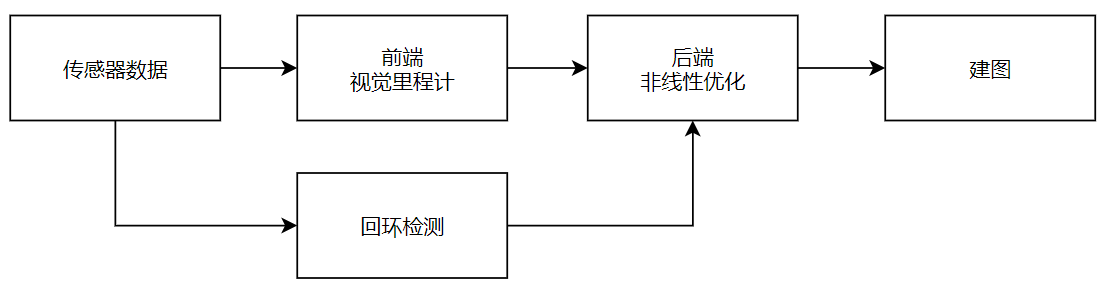
\includegraphics[width=0.8\textwidth]{figure/framework.png}
        \caption{VSLAM流程图\cite{9787121311048}}
    \end{figure}
    
\subsection{基于单个视觉传感器的V-SLAM方法}
视觉SLAM算法可根据利用图像信息的不同分为特征法(稀疏法)和直接法(半稠密法、稠密法)。
\subsubsection{特征法}
早期的单目视觉SLAM的实现是借助于滤波器而实现的\cite{9781921987243,0000001}。MonoSLAM\cite{9781921987243}是第一个实时的单目视觉SLAM系统。
MonoSLAM利用扩展卡尔曼滤波(extended Kalman filter, EKF)来实现同时定位和地图创建。但也正由于EKF的引入,
导致SLAM算法会有计算复杂度的上升以及线性化带来的不确定问题。该方法的缺点是:场景窄、路标数有限、稀疏特征点易丢失等。
\begin{figure}[H]
        \centering
        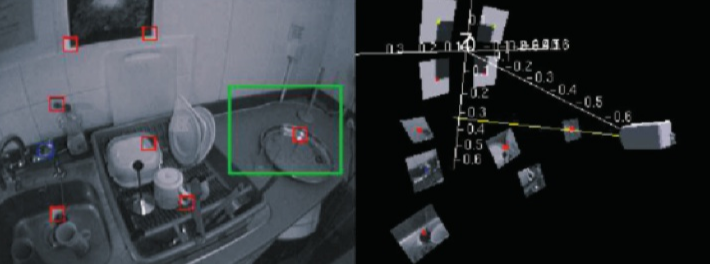
\includegraphics[width=0.7\textwidth]{figure/monoslam.png}
        \caption{MonoSLAM效果图}
\end{figure}

随后,基于关键帧的单目视觉SLAM发展起来。PTAM(parallel tracking and mapping\cite{0000002}是其中最具代表性的一个,
其首次提出了关键帧(keyframe)的概念,在保持准确度的同时,不用精细地处理每一帧,显著提高了SLAM的实时性。
同时,PTAM首次实现了跟踪和建图的并行化,区分出前后端(跟踪需要实时响应图像数据,地图优化放在后端进行),为后续的SLAM方法奠定了基本模型。
\begin{figure}[H]
        \centering
        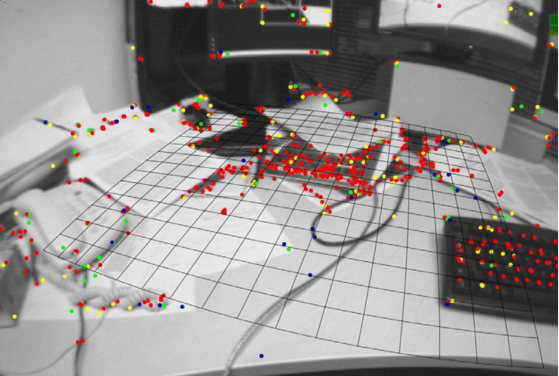
\includegraphics[width=0.5\textwidth]{figure/ptam.png}
        \caption{PTAM效果图}
\end{figure}


ORB-SLAM2算法\cite{murAcceptedTRO2015,murORB2}是首个基于单目,双目和RGB-D相机的开源SLAM方案,在大规模的、小规模的、室内室外的环境都可以运行。
其利用ORB而非SURF\cite{SURF}或者SIFT\cite{sift}特征进行运算,因此可以提高效率。同时,ORB-SLAM2又创新性地使用三个线程
完成V-SLAM(将整个流程分成定位、创建地图、闭环三个部分),得益于AMD推动了多核心CPU的发展\cite{wiki:Multi-core_processor,core_0001,core_0002},
ORB-SLAM2的三线程可以更好地发挥CPU的性能从而提高V-SLAM的实时性。


\begin{figure}[H]
        \centering
        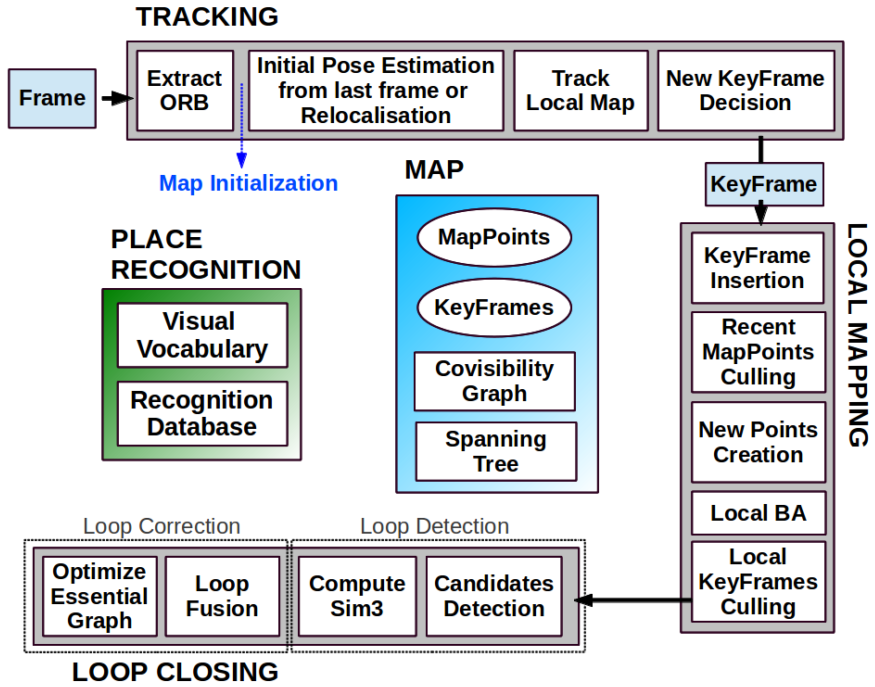
\includegraphics[width=0.5\textwidth]{figure/orb.png}
        \caption{ORB-SLAM主要分为三个线程进行,也就是如图所示的,分别是Tracking、LocalMapping和LoopClosing\cite{murORB2}}
\end{figure}
\subsubsection{直接法(稠密、半稠密)}
SVO(semi-direct monocular visual odometry)算法\cite{6906584}主要面向无人机航拍场合,它将特征点法与直接法结合,
跟踪关键点,不计算描述子,根据关键点周围的小图像块的信息估计相机的运动。主要分运动估计线程和地图构建线程两个线程。
综上所述,由于SVO的目标是无人机平台,所以其没有闭环、没有重定位、也没有建图功能,但这也使得它的实时性非常强(可以达到100FPS)。

RGBD(RGB-depth map)能够同时获得图像信息和深度信息,这大大地简化了三维重建和SLAM的过程。
随着微软公司Kinect深度相机的普及化,越来越多厂商(Intel,ZED,ASUS)也开始研制低成本、高精度的深度摄像头
这导致深度摄像头的价格开始直线下降,于是越来越多的SLAM算法开始利用深度摄像头进行研究。

RTAB-MAP开源库\cite{doi:10.1002/rob.21831}在2013年建立,直至2019年已经发展成一个跨平台的独立C++库和一个ROS包
,这说明了RTAB-MAP本质上更偏向工程应用。其通过内存管理方法来实现回环检测,同时限制了地图的大小以保证建图的实时性。
同时,通过图\ref{octo}我们可以看到RTAB-MAP开放了接口允许其他里程计数据(包括第三方视觉里程计)的接入,同时也可以选择输出:OctoMap(3D栅格地图)\cite{octomap};稠密点云地图\cite{pointcloud};
2D栅格地图\cite{6942636},对第三方VSLAM的算法评判提供了量化评判基础。
\begin{figure}[H]
        \centering
        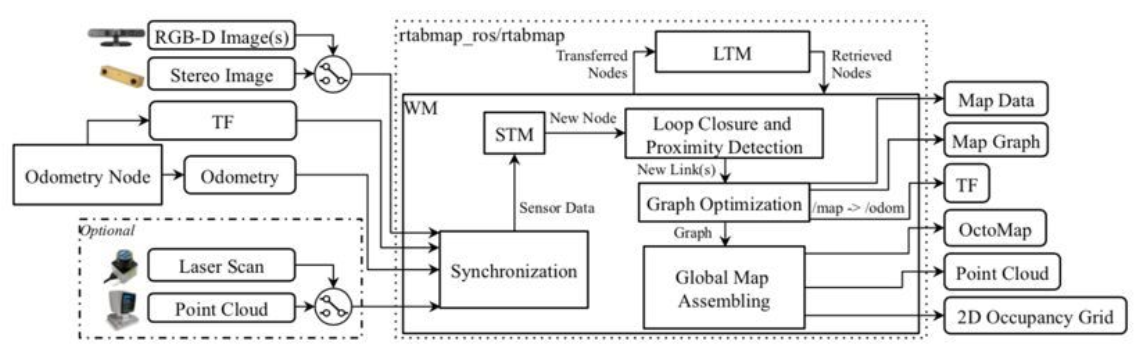
\includegraphics[width=0.9\textwidth]{figure/rtab.png}
        \caption{RTAB-Map框架}
        \label{octo}
\end{figure}
\subsubsection{经典VSLAM方法总结}
由于篇幅所限,我们无法一一列举所有VSLAM经典方法。于是我们对大部分的知名VSLAM算法概要汇总整理至表\ref{overview}。
\begin{table}[H]
        \centering
        {\footnotesize\centerline{\tabcolsep=18pt\begin{tabular*}{\textwidth}{ccccc}
                \toprule
                相关文献            &方法         & 所用传感器 & 算法名称 & 发表年份  \\
                \midrule[2pt]
                \cite{9781921987243}       &稀疏法(特征点)&       单目SLAM     &       MonoSLAM       &    2007   \\
                \cite{0000002}             &稀疏法(特征点)&       单目SLAM     &       PTAM       &    2007   \\
                \cite{10.1007/978-3-319-10605-2_54}     &半稠密法     &       单目SLAM     &       LSD-SLAM       & 2014\\
                \cite{murAcceptedTRO2015}&稀疏法(特征点)&       单目SLAM     &       ORB-SLAM       &   2015  \\
                \cite{6906584}            &半稠密法     &       单目SLAM     &       SVO        &      2014  \\
                \cite{murORB2}     &稀疏法(特征点)&       双目SLAM     &       ORB-SLAM2      &       2017  \\
                \cite{pire2015sptam}&稀疏法(特征点)&       双目SLAM     &       S-PTAM       &     2015\\
                \cite{6594910}      &稠密法       &       RGBD-SLAM     &       RGBD-SLAMv2       &   2014 \\
                \cite{doi:10.1002/rob.21831}      &稠密法       &       RGBD-SLAM     &       RTAB-SLAM       &   2019 \\
                \bottomrule
                \end{tabular*}}}
        \caption{传统 SLAM 算法的总结}
        \label{overview}
\end{table}

\subsection{多传感器融合的V-SLAM方法}

\begin{table}[H]
        \centering
        \begin{tabular}{l|ll}
        \toprule
        比较项目   &视觉里程计 & IMU里程计\\
        \midrule[2pt]
        更新频率 & 低    & 高\\
        长时间稳定性 & 高   & 低\\
        场景依赖度 & 高  &  低\\
        重定位能力 &  高  & 低\\
        CPU功耗 &  高 & 低\\
        \bottomrule
        \end{tabular}
        \caption{视觉里程计和IMU的特性对比}
\end{table}

\subsubsection{多传感器融合:VINS-Mono}
该算法\cite{8421746}是一种鲁棒且通用的单目视觉惯性状态估计器。采用一种基于紧耦合、非线性优化的方法,通过融合预积分后的IMU测量值和特征观测值,获得高精度的视觉惯性里程计。结合紧耦合方法,回环检测模块能够以最小的计算代价实现重定位。
处理视觉和惯性测量的最简单的方法是松耦合的传感器融合\cite{8576618,8630025},其中IMU被视为一个独立的模块,用于辅助运动的视觉结构(sfm)获得的纯视觉位姿估计。融合通常由扩展卡尔曼滤波(EKF)完成,其中IMU用于状态传播,而视觉位姿用于更新。
  
\textbf{IMU预积分(pre-integration)}

在实践中,IMU通常以比摄像机更高的速率获取数据。不同的方法被提出来处理高速率的IMU测量值。最简单的方法是在基于EKF的方法中使用IMU进行状态传播[11][13]。在图优化公式中,为了避免重复的IMU重复积分,提出了一种有效的方法,即IMU预积分(IMU pre-integration)。
通过一系列计算,得到下面的预积分估计值:
\begin{align} 
\hat{\boldsymbol{\alpha }}^{b_k}_{i+1} &= \hat{\boldsymbol{\alpha }}^{b_k}_i + \hat{\boldsymbol{\beta }}^{b_k}_i\delta t + \frac{1}{2} \mathbf {R}(\hat{\boldsymbol{\gamma }}^{b_k}_i)(\hat{\mathbf {a}}_i - \mathbf {b}_{a_i}) \delta t^2 \nonumber\\ \hat{\boldsymbol{\beta }}^{b_k}_{i+1} &= \hat{\boldsymbol{\beta }}^{b_k}_{i} + \mathbf {R}(\hat{\boldsymbol{\gamma }}^{b_k}_i)(\hat{\mathbf {a}}_i - \mathbf {b}_{a_i})\delta t\nonumber\\ \hat{\boldsymbol{\gamma }}^{b_k}_{i+1} &= \hat{\boldsymbol{\gamma }}^{b_k}_i \otimes {\left[\begin{array}{c}1\\ \frac{1}{2} (\hat{\boldsymbol{\omega }}_i- \mathbf {b}_{w_i})\delta t \end{array}\right]}
\end{align}
通过计算可以写下IMU测量模型所其对应的协方差${\mathbf {P}^{b_k}_{b_{k+1}}}$:
\begin{equation} 
{\left[\begin{array}{c}\hat{\boldsymbol{\alpha }}^{b_k}_{b_{k+1}}\\ \hat{\boldsymbol{\beta }}^{b_k}_{b_{k+1}}\\ \hat{\boldsymbol{\gamma }}^{b_k}_{b_{k+1}}\\ \mathbf {0}\\ \mathbf {0}\\ \end{array}\right]} = {\left[\begin{array}{c}\mathbf {R}^{b_k}_{w}(\mathbf {p}^{w}_{b_{k+1}} - \mathbf {p}^{w}_{b_k} + \frac{1}{2}\mathbf {g}^{w} \Delta t_k^2 - \mathbf {v}^{w}_{b_k} \Delta t_k) \\ \mathbf {R}^{b_k}_{w}(\mathbf {v}^{w}_{b_{k+1}} + \mathbf {g}^{w} \Delta t_k- \mathbf {v}^{w}_{b_k}) \\ \mathbf {q}^{w^{-1}}_{b_{k}} \otimes \mathbf {q}^{w}_{b_{k+1}}\\ {\mathbf {b}_a}_{b_{k+1}} - {\mathbf {b}_a}_{b_k}\\ {\mathbf {b}_w}_{b_{k+1}} -{\mathbf {b}_w}_{b_k}\\ \end{array}\right]}.
\end{equation}

\textbf{估计器初始化}

单目紧耦合VIO是一个高度非线性的系统。由于单目相机无法直接观测到尺度,因此,如果没有良好的初始值,很难直接将这两种测量结果融合在一起。
当IMU测量结果被大偏置破坏时,情况就变得更加复杂了。事实上,初始化通常是单目VINS最脆弱的步骤。需要一个鲁棒的初始化过程以确保系统的适用性。
通过对齐IMU预积分与纯视觉SfM结果,我们可以粗略地恢复尺度、重力、速度,甚至偏置。这足以引导非线性单目VINS估计器。

\begin{figure}[H]
        \centering
        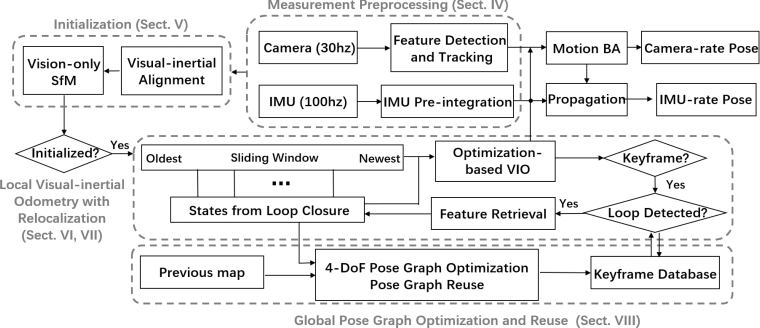
\includegraphics[width=0.6\textwidth]{figure/vins2.png}
        \caption{总体架构图}
\end{figure}

\textbf{开源代码链接:}
\url{https://github.com/HKUST-Aerial-Robotics/VINS-Mono}





\subsection{基于深度学习的V-SLAM方法}

\begin{table}[H]
        \centering
        \begin{tabular}{l|ll}
        \toprule
        比较项目   &传统SLAM算法 & 基于深度视觉的SLAM算法\\
        \midrule[2pt]
        模型参数调整难易程度 & 数据少,调参周期短    & 数据多,调参周期长\\
        魔性物理含义 & 直观意义明确   & 缺少直观意义\\
        模型泛化能力 & 信息利用不充分,泛化能力弱  &  信息利用充分,泛化能力强\\
        适应能力 &  迁移能力弱  & 迁移能力强\\
        设计流程 &  特征设计与分类训练分离 & 同步完成特征设计和分类器训练\\
        \bottomrule
        \end{tabular}
        \caption{传统 SLAM 算法与基于深度学习的 SLAM 算法对比\cite{ZHAOYang:889}}
\end{table}


%===参考文献===
\addcontentsline{toc}{section}{参考文献}
\bibliographystyle{ieeetr}     %论文引用格式:缩写
\bibliography{conference_101719} %bib文件地址
\end{document}
%===结束===



